\begin{answer}
\begin{figure}[H]
	\centering
	\begin{subfigure}[H]{0.45\linewidth}
		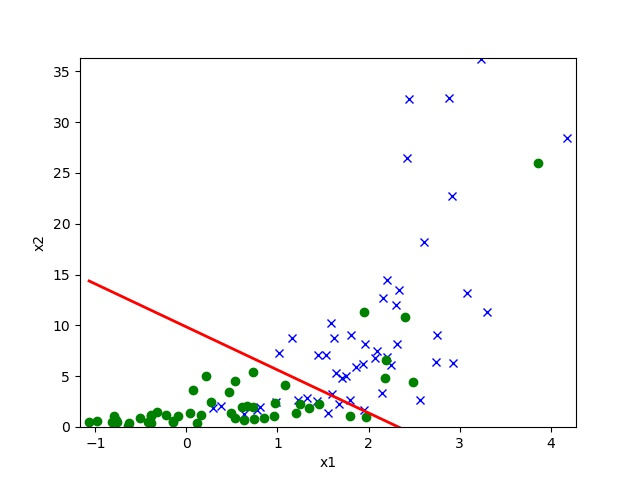
\includegraphics[width=\linewidth]{logreg_1}
		\caption{Logistic regression}
	\end{subfigure}
	\begin{subfigure}[H]{0.45\linewidth}
		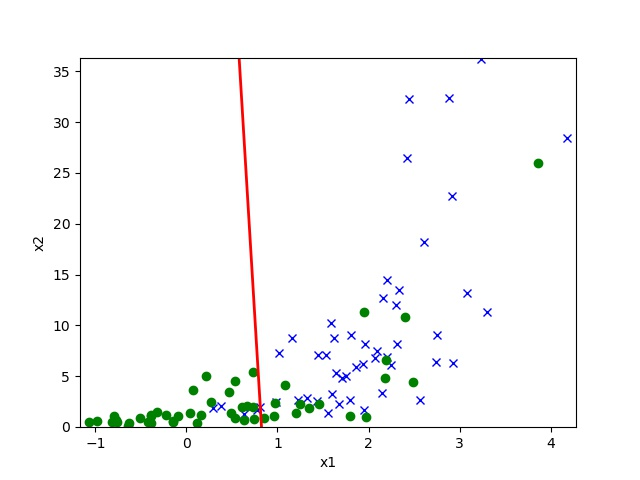
\includegraphics[width=\linewidth]{gda_1}
		\caption{GDA}
	\end{subfigure}
	\caption{Results on the Dataset 1.}
\end{figure}
In this case, the logistic regression model obtained a better decision boundary than the other. Its separating line was quite reasonable. \\	
\end{answer}
